	The front end is designed around a few simple HTML template pages, stylized with a CSS style guide. There are three main templates and a variation on two – the first template is the index, a home page that is repeatedly linked on some blank links in the navigation bar. There are also two pages dedicated to the address and weather API’s. These pages have two versions, a search and an output template. The search template uses a simple form for the user to input a URL. The output template displays the results from the API call. These files are hosted via a flask server.

	The flask server uses the render\_template and request objects to function seamlessly with the HTML and CSS. Following traditional directory organizations, a templates and static directory are used to hold those files for flask to access.
	\begin{verbatim}
	/app
    		- fServer.py
    	/templates
        - index.html
    	/static
		logo png’s
		/fonts
      	/styles
            	- style.css
	\end{verbatim}
Flask’s render\_template is used to display the correct HTML template in any given scenario, either from the hostWeather method or directly in the HTML links. The request object is used to handle the form submissions so that the user provided URL’s can be used by the API methods to generate the correct output. Both hostAddress and hostWeather use a similar method to pass the URL correctly depending on whether a POST request was made from a form submission, via requests request.form method or directly from the URL query string. From there the API methods are used to gather the data, which is the outputted using the render\_template method and displayed with in the output template.

% Include Python code snippet
\begin{lstlisting}[style=mystyle, caption=hostWeather method handles GET/POST requests, label=lst:python]

@app.route("/weather", methods=['GET', 'POST'])
def hostWeather():
    if request.method == 'POST':
        # Logic to handle form submission via POST request
        incomingHost = request.form['url']
    else:
        # Logic to handle GET request
        incomingHost = request.args.get('url', '')

    ipAddress = getIP(incomingHost)

    if checkCache(cacheW, incomingHost):
        weather = cacheW[incomingHost]
    else:
    	weather=getWeather(incomingHost)
    	addCache(cacheW, incomingHost, weather)

\end{lstlisting}

	While the host methods route to the correct output page, the remaining routes direct a user to the index or the search pages. The following sequence diagram shows the basic user interaction with the site:
\begin{figure}[htbp]
    \centering
    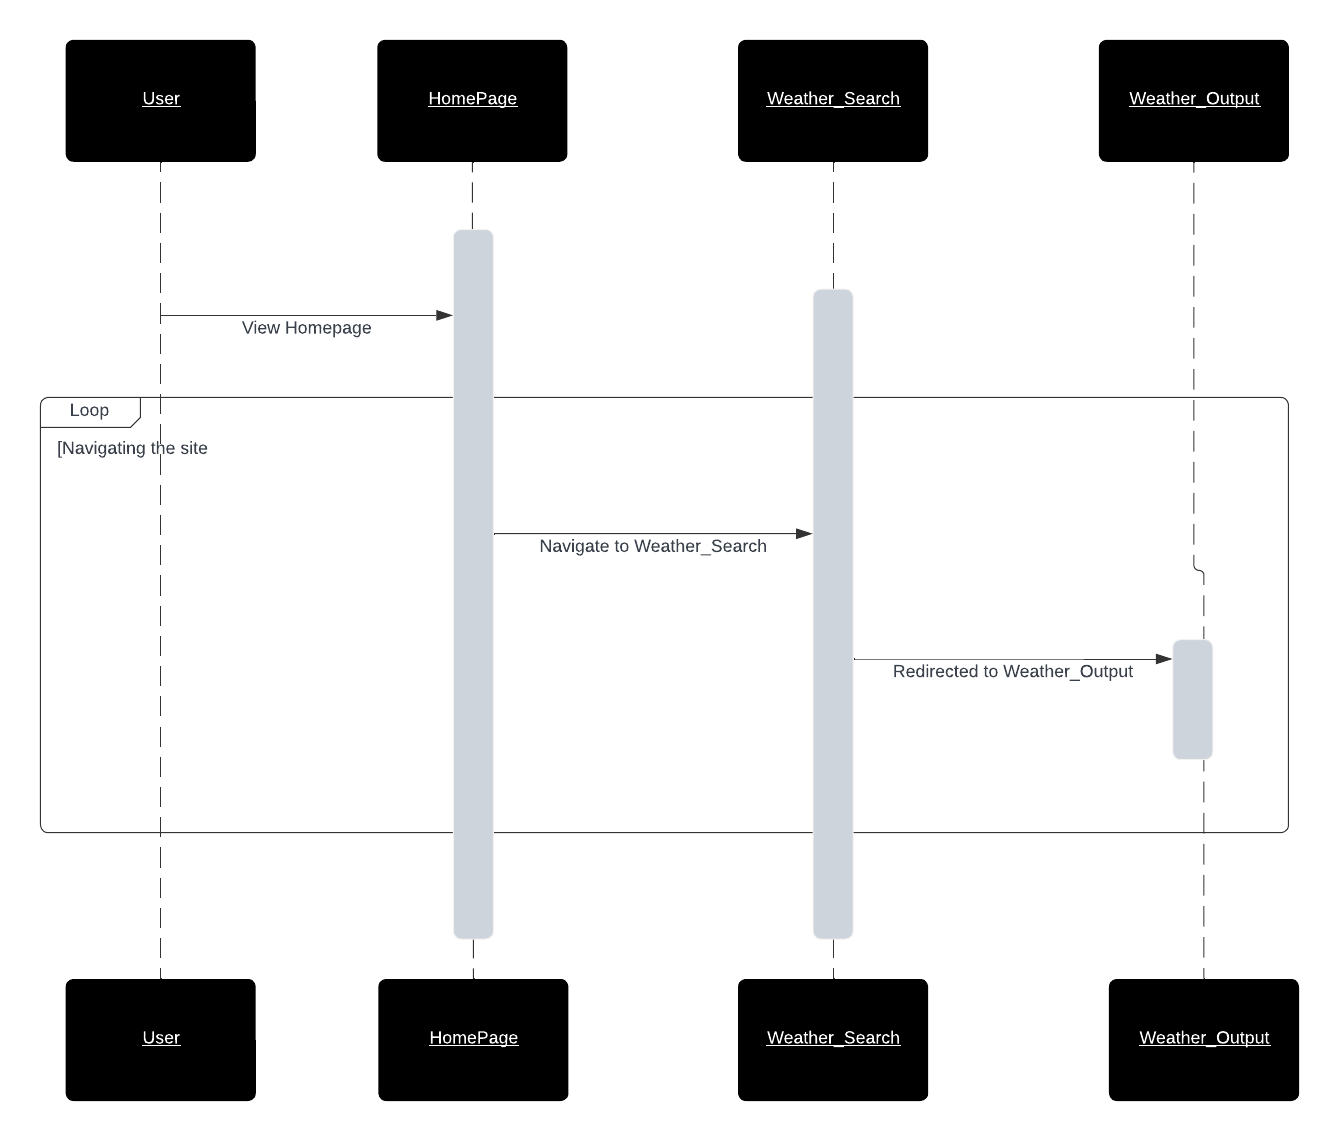
\includegraphics[width=0.5\textwidth]{sequenceD.png}
    \caption{Environment Diagram}
    \label{fig:example}
\end{figure}

	
